\documentclass[12pt]{article}
\usepackage{lecture}
\usepackage{graphicx}
\usepackage{epstopdf}
\usepackage{html}
\usepackage{url}

\newcommand{\copyrightYears}{2010-2023}

\title{Association mapping: a (very) brief overview}

\begin{document}

\maketitle

\thispagestyle{first}

\section*{Introduction}

One approach to understanding more about the genetics of quantitative
traits takes advantage of the increasing number of genetic markers
available as a result of recent advances in molecular
genetics. Suppose you have two inbred lines that differ in a trait
that interests you, say body weight or leaf width. Call one of them
the ``high'' line and the other the ``low''
line.\footnote{Corresponding to whether the body weight or leaf width
  is large or small.} Further suppose that you have a whole bunch of
molecular markers that differ between the two lines, and designate the
genotype in the ``high'' line $A_1A_1$ and the genotype in the low
line $A_2A_2$.\footnote{Since these are inbred lines, I can assume
  that they are homozygous at the marker loci I've chosen.} One last
supposition: Suppose that at loci influencing the phenotype you're
studying the genotype in the ``high'' line is $Q_1Q_1$ and the
genotype in the ``low'' line is $Q_2Q_2$. Each of these loci is what
we call a {\it quantitative trait locus\/} or QTL.\index{quantitative trait locus}\index{QTL} Now do the following experiment:

\begin{itemize}

\item Cross the ``high'' line and the ``low'' line to construct an
  $F_1$.

\item Intercross individuals in the $F_1$ generation to form an
  $F_2$.\footnote{Note: You could also backcross to either or both of
    the parental inbred lines. Producing an $F_2$, however, allows you
    to estimate both the additive and dominance effects associated
    with each QTL.}

\item ``Walk'' through the genome\footnote{I forgot to mention another
    supposition. I am supposing that you either have already
    constructed a genetic map using your markers, or that you will
    construct a genetic map using segregation in the $F_2$ before you
    start looking for QTL loci.} calculating a likelihood score for a
  QTL at a particular map position, using what we know about the
  mathematics of recombination rates and Mendelian genetics. In
  calculating the likelihood score we maximize the likelihood of the
  data assuming that there is a QTL at this position and estimating
  the corresponding additive and dominance effects of the allele. We
  then identify QTLs as those loci where there are ``significant''
  peaks in the map of likelihood scores.

\end{itemize}
The result is a genetic map showing where QTLs are in the genome and
indicating the magnitude of their additive and dominance effects.

QTL mapping is wonderful{\dash}provided that you're working with an
organism where it's possible to design a breeding program and where
the information derived from that breeding program is relevant to
variation in natural populations. Think about it. If we do a QTL
analysis based on segregation in an $F_2$ population derived from two
inbred lines, all we really know is which loci are associated with
phenotypic differences {\it between those two lines}. Typically what
we really want to know, if we're evolutionary biologists, is which
loci are associated with phenotypic differences {\it between
  individuals in the population we're studying}. That's where
association mapping comes in. We look for statistical associations
between phenotypes and genotypes across a whole population. We expect
there to be such associations, if we have a dense enough map, because
some of our marker loci will be closely linked to loci responsible for
phenotypic variation.\index{QTL mapping}

\section*{Association mapping}

So how does association mapping work? There are two broad approaches,
one that is used in genome-wide association studies (GWAS) that is
analogous to QTL mapping and one that looks for differences between
``cases,'' those that exhibit a particular phenotype of
interest~(e.g., a disease state in humans), and ``controls,'' those
that don't exhibit the phenotype of interest. Let's talk about GWAS
first.\index{Genome-wide association study}\index{case-control study}

\subsection*{Genome-wide association study}

\subsubsection*{Principles}

Imagine that we have a well-mixed population segregating both for a
lot of molecular markers spread throughout the genome and for loci
influencing a trait we're interested in, like body weight or leaf
width. Let's call our measurement of that trait $z_i$ in the $i$th
individual. Let $x_{ij}$ be the genotype of individual $i$ at the
$j$th locus.\footnote{To keep things simple I'm assuming that we're
  dealing with biallelic loci, e.g., SNPs, and we can then order the
  genotypes as 0, 1, 2 depending on how many copies of the most
  frequent allele they carry. So $x_{ij}$ is the number of copies of
  $A_1$ individual $i$ carries at locus $j$.} Then to do association
mapping, we simply fit the following regression model:
\[
y_i = x_{ij}\beta_j + \epsilon_{ij} \quad ,
\]
where $\epsilon_{ij}$ is the residual error in our regression estimate
and $\beta_j$ is our estimate of the effect of substituting one allele
for another at locus $j$, i.e., the additive effect of an allele at
locus $j$.\footnote{We can generalize the regression to allow us to
  estimate dominance effects too, but doing so only complicates the
  algebra without providing any additional insight.} If $\beta_j$ is
significantly different from 0, we have evidence that there is a locus
linked to this marker that influences the phenotype we're interested
in, and we have an estimate of the additive effect of the alleles at
that locus.

Notice that I claimed we have evidence that the locus is
linked. That's a bit of sleight of hand. I've glossed over something
very important. What we have direct evidence for is only that the
locus is {\it associated} with the phenotype differences. As we'll see
in just a bit, the observed association {\it might\/} reflect physical
linkage between the marker locus and a locus influencing the phenotype
or it could reflect a statistical association that arises for other
reasons, including population structure. So in practice the regression
model we fit is a more complicated than the one I just described. The
simplest case is when individuals fall into obvious groups, e.g.,
samples from different populations. Then $y_i^{(k)}$ is the trait
value for individual $i$. The superscript $(k)$ indicates that this
individual belongs to group $k$.
\[
y_i^{(k)} = x_{ij}\beta_j + \phi^{(k)} + \epsilon_{ij} \quad .
\]
The difference between this model and the one above is that we include
a random effect of group, $\phi^{(k)}$, to account for the fact that
individuals may have similar phenotypes not because of similarity in
genotypes at loci close to those we've scored but because of their
similarity at other loci that differ among groups. More generally, the
model looks like
\[
y_i = x_{ij}\beta_j + \phi_i + \epsilon_{ij} \quad .
\]
where $\phi_i$ is an individual random effect where the correlation
between $\phi_i$ and $\phi_j$ for individuals $i$ and $j$, i.e.,
$\rho_{ij}$, is determined by how closely related they are. The degree
of relationship might be inferred from a pedigree, if one is known, or
from coefficients of kinship estimated from a large suite of genetic
markers.

\subsubsection*{An example: warfarin maintenance
  dose}\index{genome-wide association study!warfarin}

Shortly after World War II, warfarin was introduced for use as a a rat
poison. By the mid-1950s it was approved for medical use in the United
States as a treatment for diseases in which blood clotting caused a
significant threat of stroke. It is still in common use as a treatment
for atrial fibrillation.\footnote{As it happens, my father took
  warfarin for more than 20 years before his death.} Currently, determining the
appropriate dose is done by closely monitoring the degree of
anticoagulation, an INR of
$2.5 \pm 0.5$~(\url{https://www.drugs.com/dosage/warfarin.html}). In
an effort to identify genetic markers that could be used to choose an
appropriate dosage, investigators at the University of Washington
studied the relationship between the dose of warfarin patients were
receiving and their genotype at 550,000 SNP
loci~\cite{Cooper-etal-2008}.\footnote{They log transformed warfarin
  dose (measured in milligrams per day) before the analysis.} They
identified two loci, {\it VKORC1} and {\it CYP2C9}, that were
consistently associated with warfarin dose. {\it VKORC1} encodes the
vitamin K epoxide reductaxe complex 1 enzyme, and {\it CYP2C9} encodes
a cytochrome P450~(Figure~\ref{fig:GWAS-warfarin}). Differences at
{\it VKORC1} account for approximately 25\% of the variance in
stabilized dose.\footnote{If you remembera a little human physiology,
  vitamin K may ring a bell. ``The name vitamin K comes from the
  German word
  `Koagulationsvitamin.'''~(\url{https://www.webmd.com/vitamins/ai/ingredientmono-983/vitamin-k},
  accessed 19 January 2019). Vitamin K plays an important role in
  blood clotting, so it makes sense that a locus encoding an enzyme
  related to vitamin K metabolism would have a strong association with
  the dose of warfarin needed to safely reduce blood clotting.}

\begin{figure}
\begin{center}
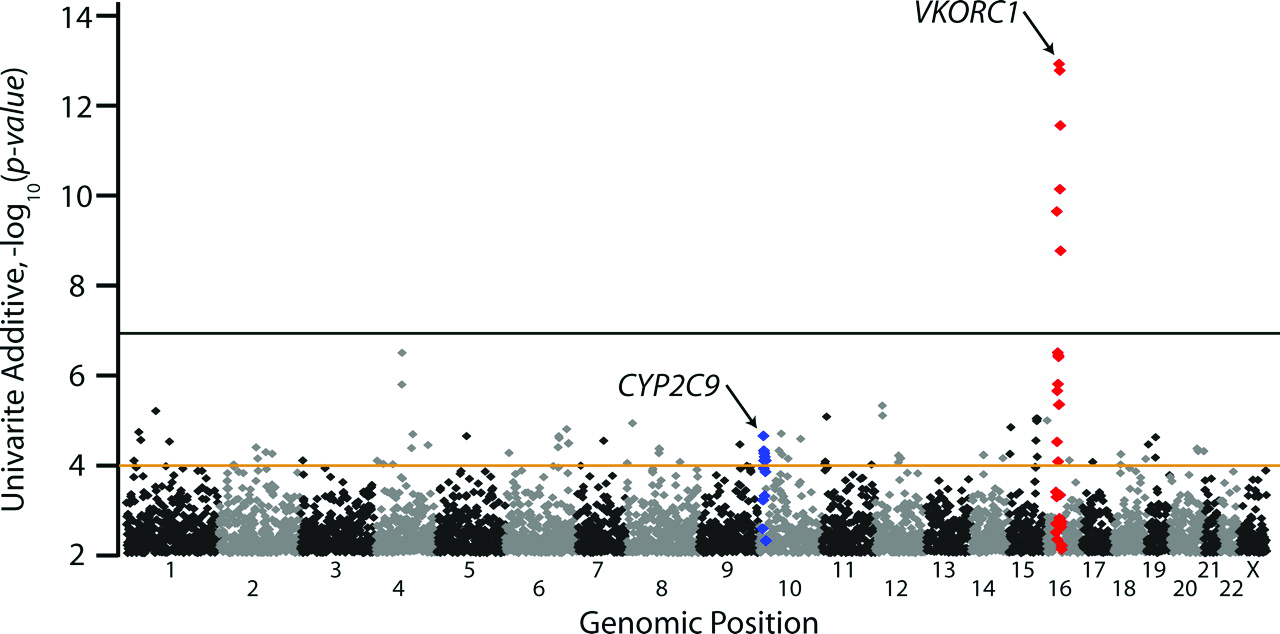
\includegraphics[height=8cm]{GWAS-warfarin.eps}
\end{center}
  \caption{$P$-values from a genome-wide analysis of the association
    between SNP genotype and warfarin dose. The black line is the
    genome-wide level for statistical significance, $10^{-7}$, and the
    brown line is the level, $10^{-4}$ at which SNPs identified in the
    index population were investigated in replicate
    populations~(from~\cite{Cooper-etal-2008}).}\label{fig:GWAS-warfarin}
\end{figure}

\subsection*{Case-control study}

The GWAS approach I just described works well if the trait we're
studying is continuous,\footnote{With the caveats about interpreting
  the association that I mentioned earlier.} but what do we do if the
trait we're interested occurs in only two states, e.g., diseased
vs. healthy? Let's suppose we have a set of ``candidate'' loci, i.e.,
loci that we have some reason to suspect might be related to
expression of the trait. Now let's suppose we divide our population
sample into two different sets: the ``cases,'' i.e., those that have
the disease,\footnote{Please note that I'm using the phrase ``have the
  disease'' merely because it's convenient. Most of the applications
  of this approach have involved investigations of human disease, but
  the approach can be used for {\it any\/} binary phenotype, in which
  case the phrase ``have the disease'' can be replaced with the phrase
  ``have the phenotype of interest.''} and the ``controls,'' i.e.,
those that don't have the disease. Let's further assume that each of
our candidate loci has only two alleles.\footnote{Just as with GWAS,
  this is a reasonable assumption, since we are probably dealing with
  SNP markers.} Then for each of our candidate loci we can estimate
the allele frequency for the population of cases, $p_{case}$, and for
the population of controls, $p_{control}$. Then we simply ask, do we
have evidence that $p_{case}$ is different from $p_{control}$. If so,
we have evidence that allelic differences at this locus are associated
with different probabilities of falling into the case category, i.e.,
allelic differences at this locus are associated with a gene that
influences development of the phenotype. As with our GWAS analysis, we
have to be careful in interpreting this association. It {\it might\/}
reflect physical linkage between the candidate locus and the gene
influencing phenotypic development or it might reflect nothing more
than a statistical association.

\section*{A digression into two-locus population
  genetics\footnote{{\bf Note}: We'll go over only a small part of
  this section in lecture. I'm providing all the details here so you
  can find them in the future if you ever need them.}}

It's pretty obvious that if two loci are on the same chromosome and
tightly linked, alleles at those loci are likely to be statistically
associated with one another, but let's take a closer look at what
being statistically associated means. We'll see that while tight
physical linkage generally implies statistical association, the
reverse isn't true. A statistical association can arise even if the
loci are unlinked and independently inherited.

One of the most important properties of a two-locus system is that it
is no longer sufficient to talk about allele frequencies alone, even
in a population that satisfies all of the assumptions necessary for
genotypes to be in Hardy-Weinberg proportions at each locus. To see
why consider this. With two loci and two alleles there are four
possible gametes:\footnote{Think of drawing the Punnett square for a
  dihybrid cross, if you want.}\index{two-locus genetics!gamet frequenies}

\begin{center}
\begin{tabular}{lcccc}
Gamete    & $A_1B_1$ & $A_1B_2$ & $A_2B_1$ & $A_2B_2$ \\
Frequency & $x_{11}$ & $x_{12}$ & $x_{21}$ & $x_{22}$
\end{tabular}
\end{center}

If alleles are arranged randomly into gametes then,
\begin{eqnarray*}
x_{11} &=& p_1p_2 \\
x_{12} &=& p_1q_2 \\
x_{21} &=& q_1p_2 \\
x_{22} &=& q_1q_2 \quad ,
\end{eqnarray*}
where $p_1 = \hbox{freq}(A_1)$ and $p_2 = \hbox{freq}(A_2)$. But
alleles need not be arranged randomly into gametes. They may covary so
that when a gamete contains $A_1$ it is more likely to contain $B_1$
than a randomly chosen gamete, or they may covary so that a gamete
containing $A_1$ is less likely to contain $B_1$ than a randomly
chosen gamete. This covariance could be the result of the two loci
being in close physical association, but as we'll see in a little bit,
it doesn't have to be. Whenever the alleles covary within gametes
\begin{eqnarray*}
x_{11} &=& p_1p_2 + D \\
x_{12} &=& p_1q_2 - D \\
x_{21} &=& q_1p_2 - D \\
x_{22} &=& q_1q_2 + D \quad ,
\end{eqnarray*}
where $D = x_{11}x_{22} - x_{12}x_{22}$ is known as the {\it gametic
  disequilibrium}.\footnote{You will usually see $D$ referred to as
  the linkage disequilibrium. I think that's misleading. Alleles at
  different loci may be non-randomly associated even when they are not
  physically linked.} When $D \ne 0$ the alleles within gametes
covary, and $D$ measures {\it statistical\/} association between
them. It does not (directly) measure the {\it physical\/}
association. Similarly, $D = 0$ does not imply that the loci are
unlinked, only that the alleles at the two loci are arranged into
gametes independently of one another.\index{gametic
  disequilibrium}\index{two-locus genetics!gametic
  disequilibrium}\index{linkage disequilibrium}

\subsection*{A little diversion}

It probably isn't obvious why we can get away with only one $D$ for
all of the gamete frequencies. The short answer is:
\begin{quote}There are four gametes. That means we need three
  parameters to describe the four frequencies. $p_1$ and $p_2$ are
  two. $D$ is the third.
\end{quote}
Another way is to do a little algebra to verify that the definition is
self-consistent.
\begin{eqnarray*}
D &=& x_{11}x_{22} - x_{12}x_{21} \\
  &=& (p_1p_2 + D)(q_1q_2 + D) - (p_1q_2 - D)(q_1p_2 - D) \\
  &=& \left(p_1q_1p_2q_2 + D(p_1p_2 + q_1q_2) + D^2\right) \\
  && \quad - \left(p_1q_1p_2q_2 - D(p_1q_2 + q_1p_2) + D^2\right) \\
  &=& D(p_1p_2 + q_1q_2 + p_1q_2 + q_1p_2) \\
  &=& D\left(p_1(p_2 + q_2) + q_1(q_2 + p_2)\right) \\
  &=& D(p_1 + q_1) \\
  &=& D \quad.
\end{eqnarray*}

\subsection*{$D$ in a finite population}

In the absence of mutation, $D$ will eventually decay to 0, although
the course of that decay isn't as regular as what is shown in the
Appendix~\cite{Hill-Robertson-1968}. If we allow recurrent mutation at
both loci, however, where\index{two-locus
  genetics!drift}\index{gametic disequilibrium!drift}
\[
\begin{array}{ccccccc}
    &\mu_1            &     &      &     &\mu_2 \\
A_1 &\rightleftharpoons& A_2 &\qquad& B_1 &\rightleftharpoons& B_2
\quad , \\
    &\nu_1            &     &      &     &\nu_2
\end{array}
\]
then it can be shown~\cite{Ohta-Kimura-1969} that the expected value
of $D^2/p_1(1-p_1)p_2(1-p_2)$ is
{\scriptsize
\begin{eqnarray*}
\frac{\mbox{E}(D^2)}{\mbox{E}(p_1(1-p_1)p_2(1-p_2))}
&=& \frac{1}{3 + 4N_e(r+\mu_1+\nu_1+\mu_2+\nu_2)
                           - \frac{2}{(2.5 + N_e(r+\mu_1+\nu_1+\mu_2+\nu_2)
                              + N_e(\mu_1+\nu_1+\mu_2+\nu_2))}} \\
&\approx& \frac{1}{3 + 4N_er} \quad .
\end{eqnarray*}}
Bottom line: In a finite population, we don't expect $D$ to go to 0,
and the magnitude of $D^2$ is inversely related to amount of
recombination between the two loci. The less recombination there is
between two loci, i.e., the smaller $r$ is, the larger the value of
$D^2$ we expect.

This has all been a long way\footnote{OK. You can say it. A {\bf\it
    very\/} long way.} of showing that our initial intuition is
correct. If we can detect a statistical association between a marker
locus and a phenotypic trait, it suggests that the marker locus and a
locus influence expression of the trait are physically linked. {\it
  But\/} we have to account for the effect of population structure,
{\it and\/} we have to account for the effect of {\it past\/}
population structure.\footnote{I haen't told you why we need to
  account for population structure, but you'll see in just a moment.}
Notice also that if the effective population size is large, $D^2$ may
be very small unless $r$ is very small, meaning that you may need to
have a very dense genetic map to detect any association between any of
your marker loci and loci that influence the trait you're studying. As
shown in the Appendix, it takes a while for the statistical
association between loci to decay after two distinct populations
mix. So if we are dealing with populations having a history of
hybridization, teasing apart physical linkage and statistical
association can become very challenging.\footnote{Think about what
  this means for GWAS or case-control studies in human populations.}

\section*{Population structure with two loci}

You can probably guess where this is going. With one locus I showed
you that there's a deficiency of heterozygotes in a combined sample
even if there's random mating within all populations of which the
sample is composed. The two-locus analog is that you can have gametic
disequilibrium in your combined sample even if the gametic
disequilibrium is zero in all of your constituent
populations. Table~\ref{table:d-structure} provides a simple numerical
example involving just two populations in which the combined sample
has equal proportions from each population.\index{Wahlund effect!two loci}

\begin{table}
\begin{center}
\begin{tabular}{c|cccc|cc|c}
\hline\hline
           & \multicolumn{4}{c|}{Gamete frequencies}
           & \multicolumn{2}{c|}{Allele frequencies} \\
Population & $A_1B_1$ & $A_1B_2$ & $A_2B_1$ & $A_2B_2$
           & $p_{i1}$ & $p_{i2}$ & $D$ \\
\hline
1          & 0.24     & 0.36     & 0.16    & 0.24
           & 0.60     & 0.40     & 0.00 \\
2          & 0.14     & 0.56     & 0.06    & 0.24
           & 0.70     & 0.20     & 0.00 \\
Combined   & 0.19     & 0.46     & 0.11    & 0.24
           & 0.65     & 0.30     & -0.005 \\
\hline
\end{tabular}
\end{center}
\caption{Gametic disequilibrium in a combined population
  sample.}\label{table:d-structure}
\end{table}

\subsection*{The gory details}

You knew that I wouldn't be satisfied with a numerical example, didn't
you? You knew there had to be some algebra coming, right? Well, here
it is. Let
\begin{eqnarray*}
D_i &=& x_{11,i} - p_{1i}p_{2i} \\
D_t &=& \bar x_{11} - \bar p_1\bar p_2 \quad ,
\end{eqnarray*}
where $\bar x_{11} = \frac{1}{K} \sum_{k=1}^K x_{11,k}$, $\bar p_1 =
\frac{1}{K} \sum_{k=1}^K p_{1k}$, and $\bar p_2 = \frac{1}{K}
\sum_{k=1}^K p_{2k}$. Given these definitions, we can now calculate
$D_t$.
\begin{eqnarray*}
D_t &=& \bar x_{11} - \bar p_1\bar p_2 \\
    &=& \frac{1}{K} \sum_{k=1}^K x_{11,k} - \bar p_1\bar p_2 \\
    &=& \frac{1}{K} \sum_{k=1}^K (p_{1k}p_{2k} + D_k) - \bar p_1\bar p_2 \\
    &=& \frac{1}{K} \sum_{k=1}^K (p_{1k}p_{2k} - \bar p_1\bar p_2) + \bar D \\
    &=& \mbox{Cov}(p_1, p_2) + \bar D \quad ,
\end{eqnarray*}
where $\mbox{Cov}(p_1, p_2)$ is the covariance in allele frequencies
across populations and $\bar D$ is the mean within-population gametic
disequilibrium. Suppose $D_i = 0$ for all subpopulations. Then $\bar D
= 0$, too (obviously). But that means that
\begin{eqnarray*}
D_t &=& \hbox{Cov}(p_1, p_2) \quad .
\end{eqnarray*}
So if allele frequencies covary across populations, i.e.,
$\mbox{Cov}(p_1, p_2) \ne 0$, then there will be non-random
association of alleles into gametes in the sample, i.e., $D_t \ne 0$,
even if there is random association alleles into gametes within each
population.\footnote{Well, duh! Covariation of allele frequencies
  across populations means that alleles are non-randomly associated
  across populations. What other result could you possibly expect?}

Returning to the example in Table~\ref{table:d-structure}
\begin{eqnarray*}
\mbox{Cov}(p_1, p_2) &=& 0.5(0.6-0.65)(0.4-0.3) + 0.5(0.7-0.65)(0.2-0.3) \\
                     &=& -0.005 \\
\bar x_{11}          &=& (0.65)(0.30) - 0.005 \\
                     &=& 0.19 \\
\bar x_{12}          &=& (0.65)(0.7) + 0.005 \\
                     &=& 0.46 \\
\bar x_{21}          &=& (0.35)(0.30) + 0.005 \\
                     &=& 0.11 \\
\bar x_{22}          &=& (0.35)(0.70) - 0.005 \\
                     &=& 0.24 \quad .
\end{eqnarray*}

\subsection*{Implications for GWAS}

For GWAS this means that we have to be very careful to account for
{\it any\/} population structure within our data if we want to
interpret a {\it statistical\/} association between a locus and a
trait as indicating that the locus is {\it physically\/} associated
with a locus influencing expression of the trait. In the example
you'll work through in lab we do this by including an estimate of the
genetic relatedness of individuals in our sample in the regression
model. Specifically, in this regression equation
\[
  y_i = x_{ij}\beta_j + \phi_i + \epsilon_{ij} 
\]
$\epsilon$ is pure random error with a mean of 0 and a variance equal
to the environmental variance. $\phi_i$ is a correlated error in which
the residual for individual $i$ is correlated with the residual for
individual $j$ and the degree of correlation is related to the degree
of relationship between them.

\bibliography{popgen}
\bibliographystyle{plain}

\section*{Appendix: Transmission genetics with two loci}

I'm going to construct a reduced version of a mating table to see how
gamete frequencies change from one generation to the next. There are
ten different two-locus genotypes (if we distinguish coupling,
$A_1B_1/A_2B_2$, from repulsion, $A_1B_2/A_2B_1$, heterozygotes as we
must for these purposes). So a full mating table would have 100
rows. If we assume all the conditions necessary for genotypes to be in
Hardy-Weinberg proportions apply, however, we can get away with just
calculating the frequency with which any one genotype will produce a
particular gamete.\footnote{We're assuming random union of {\it
    gametes\/} rather than random mating of {\it
    genotypes}.}\index{two-locus genetics!transmission}

\begin{center}
\begin{tabular}{lccccc}
\hline\hline
         &           & \multicolumn{4}{c}{Gametes} \\
Genotype & Frequency & $A_1B_1$ & $A_1B_2$ & $A_2B_1$ & $A_2B_2$ \\
\hline
$A_1B_1/A_1B_1$ & $x_{11}^2$ & 1 & 0 & 0 & 0 \\
$A_1B_1/A_1B_2$ & $2x_{11}x_{12}$ & $\half$ & $\half$ & 0 & 0 \\
$A_1B_1/A_2B_1$ & $2x_{11}x_{21}$ & $\half$ & 0 & $\half$ & 0 \\
$A_1B_1/A_2B_2$ & $2x_{11}x_{22}$ & \oneminus & \rhalf & \rhalf & \oneminus \\
$A_1B_2/A_1B_2$ & $x_{12}^2$ & 0 & 1 & 0 & 0 \\
$A_1B_2/A_2B_1$ & $2x_{12}x_{21}$ & \rhalf & \oneminus & \oneminus & \rhalf \\
$A_1B_2/A_2B_2$ & $2x_{12}x_{22}$ & 0 & $\half$ & 0 & $\half$ \\
$A_2B_1/A_2B_1$ & $x_{21}^2$ & 0 & 0 & 1 & 0 \\
$A_2B_1/A_2B_2$ & $2x_{21}x_{22}$ & 0 & 0 & $\half$ & $\half$ \\
$A_2B_2/A_2B_2$ & $x_{22}^2$ & 0 & 0 & 0 & 1 \\
\hline
\end{tabular}
\end{center}

\subsection*{Where do $\frac{1-r}{2}$ and $\frac{r}{2}$ come from?}

Consider the coupling double heterozygote, $A_1B_1/A_2B_2$. When
recombination doesn't happen, $A_1B_1$ and $A_2B_2$ occur in equal
frequency ($1/2$), and $A_1B_2$ and $A_2B_1$ don't occur at all. When
recombination happens, the four possible gametes occur in equal
frequency ($1/4$). So the recombination frequency,\footnote{The
  frequency of recombinant gametes in double heterozygotes.} $r$, is
half the crossover frequency,\footnote{The frequency of cytological
  crossover during meiosis.} $c$, i.e., $r = c/2$. Now the results of
crossing over can be expressed in this table:\index{two-locus genetics!recombination}\index{recombination frequency}

\begin{center}
\begin{tabular}{c|cccc}
\hline\hline
Frequency & $A_1B_1$ & $A_1B_2$ & $A_2B_1$ & $A_2B_2$ \\
\hline
$1-c$     & $\half$  & 0        & 0        & $\half$ \\
$c$       & $\quarter$ & $\quarter$ & $\quarter$ & $\quarter$ \\
\hline
Total     & $\frac{2-c}{4}$ & $\frac{c}{4}$ & $\frac{c}{4}$
          & $\frac{2-c}{4}$ \\
          & $\frac{1-r}{2}$ & $\frac{r}{2}$ & $\frac{r}{2}$
          & $\frac{1-r}{2}$ \\
\hline
\end{tabular}
\end{center}

\subsection*{Changes in gamete frequency}

We can use the mating table table as we did earlier to calculate the
frequency of each gamete in the next generation. Specifically,
\begin{eqnarray*}
x_{11}' &=& x_{11}^2 + x_{11}x_{12} + x_{11}x_{21} + (1-r)x_{11}x_{22}
            + rx_{12}x_{21} \\
        &=& x_{11}(x_{11} + x_{12} + x_{21} + x_{22})
            - r(x_{11}x_{22} - x_{12}x_{21}) \\
        &=& x_{11} - rD \\
x_{12}' &=& x_{12} + rD \\
x_{21}' &=& x_{21} + rD \\
x_{22}' &=& x_{22} - rD \quad .
\end{eqnarray*}

\subsection*{No changes in allele frequency}

We can also calculate the frequencies of $A_1$ and $B_1$ after this
whole process:
\begin{eqnarray*}
p_1' &=& x_{11}' + x_{12}' \\
     &=& x_{11} - rD + x_{12} + rD \\
     &=& x_{11} + x_{12} \\
     &=& p_1 \\
p_2' &=& p_2 \quad .
\end{eqnarray*}
Since each locus is subject to all of the conditions necessary for
Hardy-Weinberg to apply at a single locus, allele frequencies don't
change at either locus. Furthermore, genotype frequencies at each
locus will be in Hardy-Weinberg proportions. But the two-locus gamete
frequencies change from one generation to the next.\index{two-locus genetics!Hardy-Weinberg}

\subsection*{Changes in $D$}

You can probably figure out that $D$ will eventually become zero, and
you can probably even guess that how quickly it becomes zero depends
on how frequent recombination is. But I'd be astonished if you could
guess exactly how rapidly $D$ decays as a function of $r$.  It takes a
little more algebra, but we can say precisely how rapid the decay will
be.\index{two-locus genetics!decay of disequilibrium}
\begin{eqnarray*}
D' &=& x_{11}'x_{22}' - x_{12}'x_{21}' \\
   &=& (x_{11} - rD)(x_{22} - rD) - (x_{12} + rD)(x_{21} + rD) \\
   &=& x_{11}x_{22} - rD(x_{11} + x_{12}) + r^2D^2
       - (x_{12}x_{21} + rD(x_{12} + x_{21}) + r^2D^2) \\
   &=& x_{11}x_{22} - x_{12}x_{21} - rD(x_{11} + x_{12} + x_{21} + x_{22}) \\
   &=& D - rD \\
   &=& D(1-r)
\end{eqnarray*}
Notice that even if loci are unlinked, meaning that $r = 1/2$, $D$
does not reach 0 immediately. That state is reached only
asymptotically. The two-locus analogue of Hardy-Weinberg is that
gamete frequencies will {\it eventually\/} be equal to the product of
their constituent allele frequencies.

\ccLicense

\end{document}



